\documentclass[12pt]{article}

\usepackage{times}
\usepackage{amssymb,amsmath}
\usepackage{graphicx}
\usepackage{subfigure}
%\usepackage{verbatim}
\usepackage{hyperref}
%\usepackage{doublespace}
%\usepackage{lineno}

%-------------- editing ----------------------
\usepackage{color}
\newcommand{\comment}[1]{\textcolor{blue}{[ \sc{#1} ]}} % comments
\newcommand{\revise}[1]{\textcolor{black}{{#1}}} % revisions
%\usepackage{ulem}
%---------------------------------------------

\begin{document}
%\linenumbers

\title{
Vehicular Mobility in San Francisco
}

\author{Jonathan W. Lee}

\date{\today}

\maketitle

\section{Motivation}
As urbanization, vehicular dependence, and fuel consumption continue to grow into the future, mobility within cities becomes an increasingly relevant dilemma. Large metropolitan areas like Los Angeles, New York City, and Washington, D.C. are notorious for terrible traffic conditions. Los Angeles conditions are particularly problematic as many carpool lanes are in effect 24/7, as opposed to the typical rush hour period in most cities. Traffic has direct impacts on commute times, road safety, energy consumption and dependence, etc., not to mention countless intangible impacts. This project is aimed at evaluating the traffic problem from a mobility perspective.

\section{Introduction}

In my preliminary work, I have found a dataset which contains archived anonymized GPS traces from Uber -- time of day, day of week, latitude, and longitude of 25,000 trips in San Francisco, logged every four seconds. The data has been anonymized by truncating the beginning and end of every trip and removing the actual dates of the trips.

\begin{figure}[hbtp]
\caption{\label{fig:overlay}An overlay of Uber GPS traces in San Francisco.}
\begin{center}
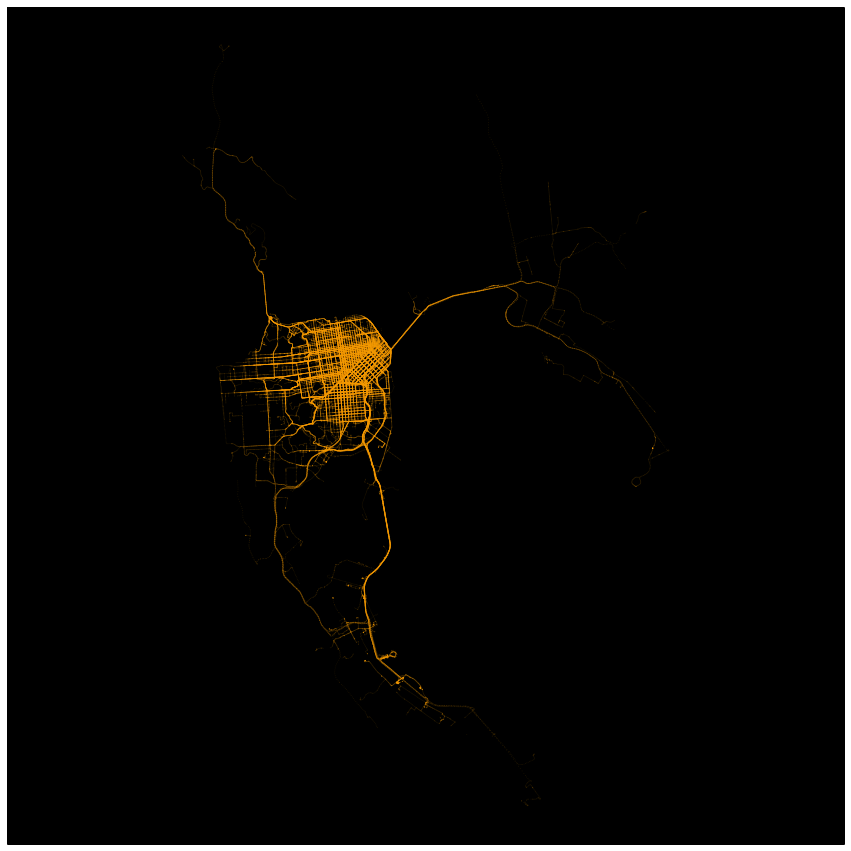
\includegraphics[width=5in]{overlay_uber.png}
\end{center}
\end{figure}

From this dataset, my goal is to obtain a better understanding of different driving behaviors in San Francisco, and how they may affect fuel economy and travel times. I plan to characterize driving behaviors in the city of San Francisco as a function of day of week, time of day, and location. Additionally, I would like to develop a model to predict fuel consumption. To achieve these goals, I will need to derive several intermediary variables from those provided in the data sets:

\begin{itemize}
\item traffic: create a model of standard traffic for all roads given weekday/weekend and hour of the day using Uber and SFMTA data
\item Driver velocity: time derivative of position, using central differences method
\item Driver acceleration: second time derivative of position
\end{itemize}

\section{Data Project}

With the above variables established, I propose three potential deliverables, each compounding upon the previous.

\begin{enumerate}

\item \textbf{Deliverable 1}: First, I will use \textit{k}-means and/or hierarchical clustering to categorize driver behavior. This project provides a quantifiable, deterministic approach to categorize an abstract concept like driving behavior. Further, it allows us to simply correlate an abstract concept (driver behavior) with concrete numerical quantities (\textit{e.g.}, energy consumption, Uber driver rating, travel time, etc.).

Clustering will be based on features engineered out of the variables listed above (\textit{e.g.}, maximum velocity, median velocity, maximum acceleration, maximum deceleration, etc.). In order to normalize out traffic conditions, perhaps the time series will be modified by the standard traffic model, mentioned above. Alternatively, this can be performed separately for rush-hour and non-rush-hour times.

To prototype how this categorization may prove useful, I will also create a rudimentary model for fuel consumption, which will be approximately proportional to an integral of positive accelerations. Alternatively, for electrified vehicles, electricity consumption may also be computed by subtracting some integral of negative accelerations to model regenerative braking. It may also be influenced by topography (\textit{e.g.}, accelerating uphill, regenerating downhill, etc.). This will allow me to find the relationship (if any) between categorized driving behaviors and fuel economy.

\item \textbf{Deliberable 2}: I will build a routing algorithm, given starting location, destination, day of week, time of day, and driving behavior. The base algorithm will use Dijkstra's algorithm, however it will be modified to present multiple route options, \textit{e.g.}, fastest route, most direct, best fuel economy, least congestion, etc. This will also serve as a prototype for a potential future product, where a user looking for directions will be also be given predicted energy consumption and travel time, etc. customized to the user.

\item \textbf{Deliberable 3} (unlikely): I will build a mobility map of San Francisco. The tool will take as inputs starting location, day of week, time of day, travel time, and driving behavior (based on the clustering in Project 1). As output, it will present a highlighted area of all potential destinations that are reachable in the given travel time. Versions of this have already been implemented, \textit{i.e.}, Isoscope and Trulia. However, Isoscope is limited to 10 minute trips, Trulia has no time dependence feature (presumably limited to commute hours), and neither factor in driving behavior. Additionally, my tool will report (via color) the fuel/electricity consumed for all destinations at the boundary. To find the potential destinations, I will use some modified form of Dijkstra's algorithm. Cumulative travel time and consumed fuel will be tracked as the algorithm proceeds.

\end{enumerate}

\section{Preliminary Work}

From the Uber dataset, I have derived velocity and acceleration time series for each driver using a central differences method. An example of one extracted time series can be found \href{https://b7097c28bb33c303afec66e136e388566fb53b52.googledrive.com/host/0Bz6ioWtHYtNJVjJacklTdHQ2cGM/}{here} (top to bottom: position, speed, acceleration time series).

Further, simple features have been extracted from these time series, such as maximum velocity, median velocity, mean velocity, maximum acceleration, median acceleration, mean acceleration, maximum deceleration, median deceleration, mean deceleration, and mean free path. The mean free path is a metric crudely approximated by averaging the duration of driving between successive pauses in a route (\textit{i.e.}, the time between zero-velocity and zero-velocity).

\begin{figure}[hbtp]
\caption{\label{fig:features}An overview of preliminary features.}
\begin{center}
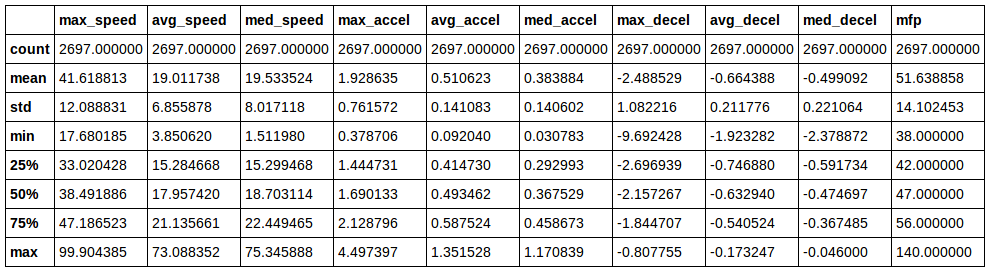
\includegraphics[width=5.5in]{feature_describe.png}
\end{center}
\end{figure}

These ten simple features have been used to build a hierarchical clustering dendrogram. Due to some noisy data, a large majority of rides had to be removed for this preliminary study. The resulting dendrogram shows four clusters of slightly varying radii.

\begin{figure}[hbtp]
\caption{\label{fig:dendrogram}Preliminary dendrogram.}
\begin{center}
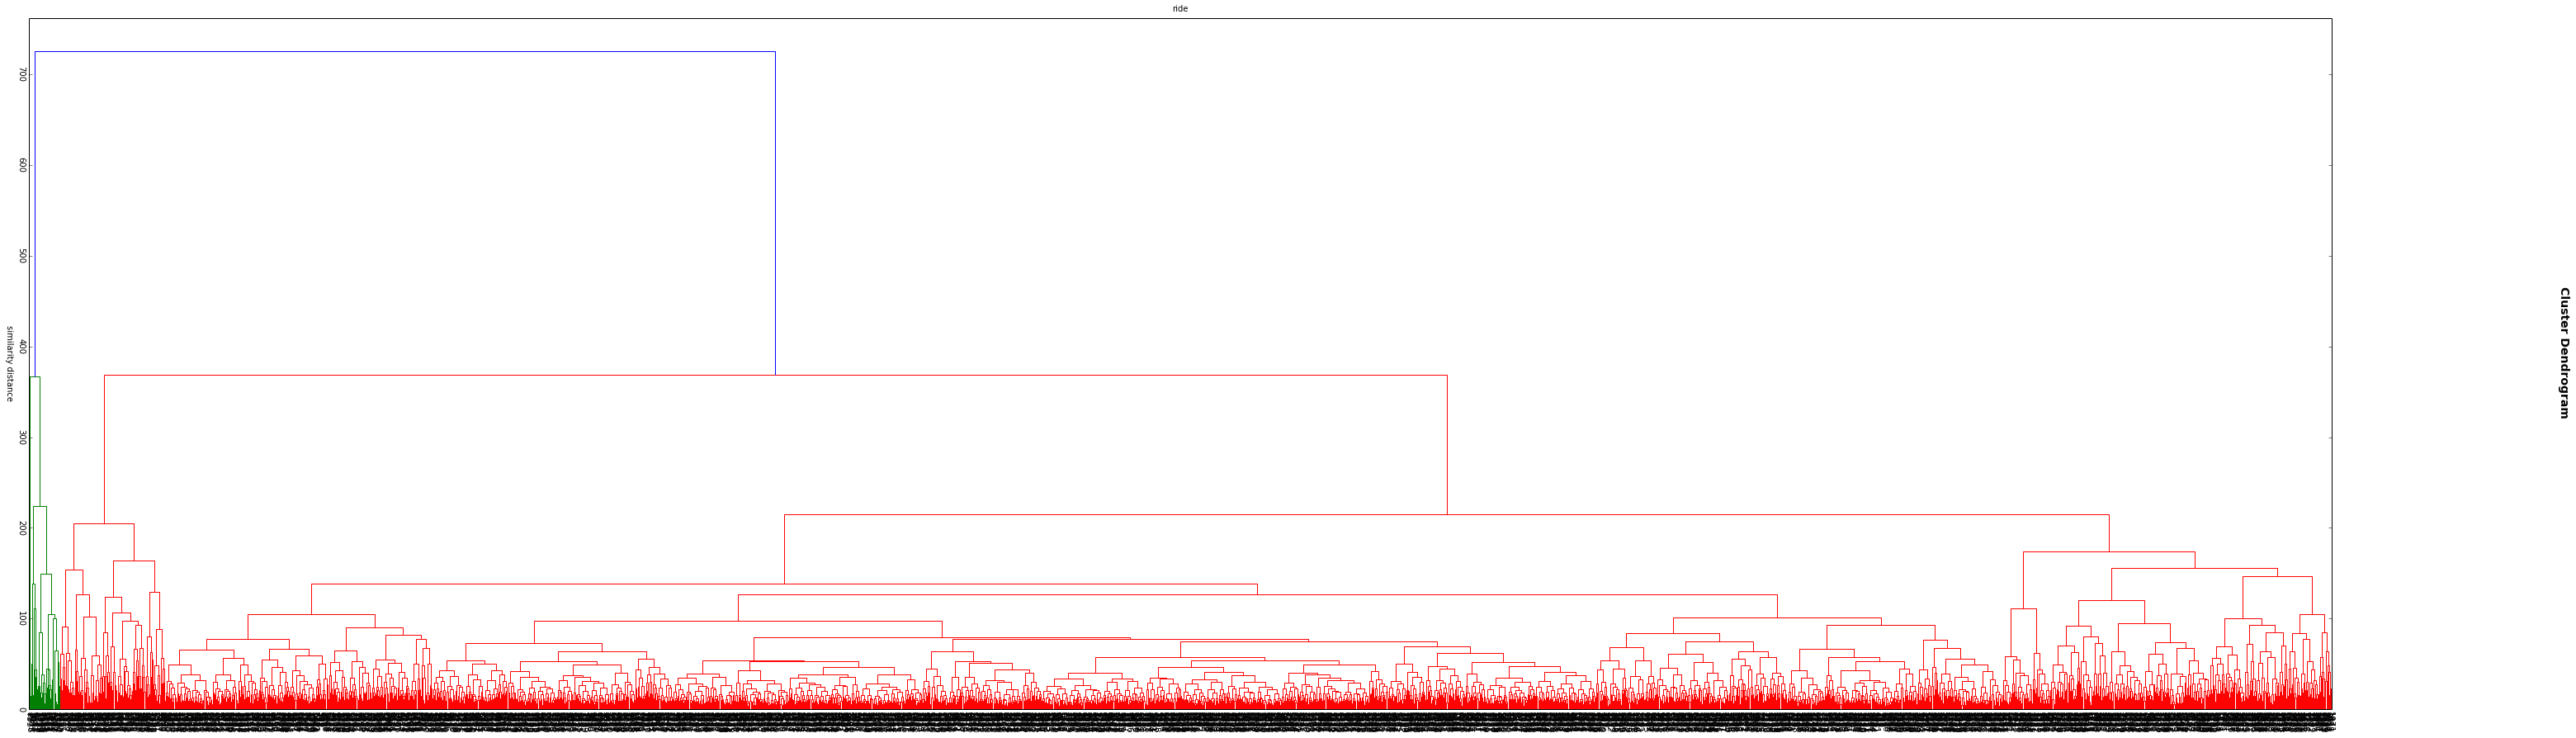
\includegraphics[width=5.5in]{dendro.png}
\end{center}
\end{figure}

\section{Challenges Ahead}

Here are four initial foreseeable challenges and my approach to addressing them:

\begin{enumerate}
\item \textbf{Extract Dendrogram Clusters}: Since the dendrogram clusters are potentially of varying size, it is somewhat difficult to inspect the clusters. If scipy does not provide a feasible way to do this, one solution is to switch to \textit{k}-means. Alternatively, I could implement my own hierarchical clustering, which will have the required functionality to inspect variable-sized clusters.
\item \textbf{Noisy Data}: I have two solutions for this which could be used unison. The first is a Kalman Filter, which should smooth out the positional data. The second is mapping GPS coordinates onto streets. This will require building a graph of intersections (nodes) and streets (edges) of San Francisco, using SF street lines shape files. Mapping might be done through a process of voting, where successive time series points will vote on the street.
\item \textbf{Normalize Out Traffic}: This will require the graph/mapping solution from the previous challenge. With the time series mapped onto streets, I can find average time series per edge per time window (perhaps every one hour window). Normalizing would then be some comparison between individual time series per edge to average time series per edge. I will consider subtraction, division, Z-scoring, and maybe others.
\item \textbf{Fuel Economy}: I need to build a model for fuel usage. This will be a function of integrating positive accelerations. For now, the model will not be based on concrete data since vehicle performance is unknown.
\end{enumerate}


% In addition to the above dataset, I may also include sources from topography data, SF street lines, and/or SF traffic shape files. It would also be nice to include influences from 
% weather, but correlation with the Uber data may be difficult since the Uber data has been anonymized (\textit{i.e.}, dates are modified).


\section{Alternate Project}

As a backup project, I might use data from my previous research in molecular simulations of supercapacitors. I have tens of thousands of atom trajectories over millions of timesteps for multiple combinations of parameters (\textit{i.e.}, surface charge density, atomic constituents, surface substrate material, etc.). Atomic and molecular arrangement and orientation turn out to be key to determining a system's capacitance, but are highly susceptible to the substrate lattice. I can use the data to build a model for predicting substrate, given a subset of ionic and solvent locations. If possible, it will be a generative model which will be able to generate atom locations given a particular substrate and surface charge density.

\end{document}
